\section{Requirements}
This chapter describes how to arrange and write a Red Book compatible audio CD. Traverso uses \texttt{cdrdao} to actually write the CD, so this program must be installed on the system. \texttt{cdrdao} is available from the official repositories of all  major and up-to-date Linux distributions, it is thus recommended to install it via the distribution's package manager. The Windows and Mac OS X installer takes care of installing cdrdao for you, so if you are on one of these platforms, you skip this section!

\footnotesize
\begin{verbatim}
tux@linux:~$ cdrdao

Cdrdao version 1.2.2 - (C) Andreas Mueller <andreas@daneb.de>
  SCSI interface library - (C) Joerg Schilling
  Paranoia DAE library - (C) Monty

Check http://cdrdao.sourceforge.net/drives.html#dt for current 
driver tables.


Usage: cdrdao <command> [options] [toc-file]
command:
...
\end{verbatim}
\normalsize

If the command was not found, the next section explains how to install \texttt{cdrdao} on the Linux platform.

\subsection{Linux}
Installing \texttt{cdrdao} on Linux is straight forward, since it is part of all major distributions. Use your distribution's package manager (e.\,g. Synaptic or Adept on (K)Ubuntu, Yast on SuSE), search for \texttt{cdrdao} and install the binary package. Alternatively, you can install it from a terminal. The commands will differ depending on the distribution. For (K,X)Ubuntu, enter the following lines in a terminal:

\begin{verbatim}
sudo apt-get update
sudo apt-get install cdrdao
\end{verbatim}


\section{Tracks and Markers}
There are basically two ways of defining tracks for a CD. Each sheet can be a track, or the entire CD can be arranged in the timeline of a sheet and tracks are defined by markers. Combinations of the two ways are also possible. Let's have a closer look at these two concepts.

\subsection{A Sheet is a CD-Track}
As you may have noticed, Traverso allows to have several sheets in a project. Some people like this feature, as one can combine all sheets of an album in one project, and still focus on one sheet at a time. If you want to write a CD containing all sheets of your project, make sure you check the ``All sheets'' button in the export dialogue. Each sheet will be rendered to a track, from position 00:00:00 up to the end of the last audio clip, and consequently each sheet will become a track on the CD.

\subsection{CD in a timeline}
Sometimes it is important to fine-tune the transition from one track to the next, e.\,g. by adding a little bit of silence in between, or by fading the previous track into the next one. In that case it can be easier to arrange the entire CD in one timeline and split it into tracks using markers. Let's look at an example in order to show how this works. (Look at \FigT~\ref{fig_markers01} if you get lost with the explanations.) Open or create a project with only two audio clips. Suppose we want clip 1 to be track 1 on the CD, and clip 2 will be track 2. Position them on the first and maybe second track, starting at position 00:00:00, as you want to hear them on the CD. Leave some silence between the end of clip 1 and the beginning of clip 2. To get Traverso to start a new CD track there, position the mouse cursor on the gap between the two clips, and press \sact{M}. This adds a small triangle to the timeline at the position of the mouse cursor, and two more at position 00:00:00 and at the end of clip 2. The latter one is labelled ``End'', and it marks the end of the CD. You can shift it a bit further back if you don't want the CD to stop right there (remember you  can have reverb tails extending beyond the last audio sample, which you don't want to cut off).

\begin{figure}[t]
 \centering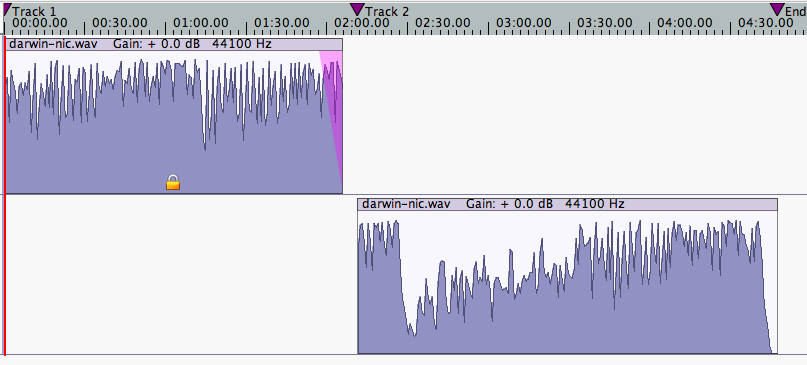
\includegraphics[width=\textwidth]{images/markers01}
 \caption{If a CD is arranged in one sheet, markers can be used to define CD tracks. Always keep the ones at position 00:00:00 and at the end.}
 \label{fig_markers01}
\end{figure}

These triangles are CD track markers, and they can be moved, added, and deleted freely (press \sact{Q} on the timeline to list all available functions.) However, it is also possible to create setups which don't make sense. E.\,g. only having one track marker in the timeline. In such cases, Traverso tries to guess the most sensible solution, and adds markers on the fly at positions it considers appropriate (which is usually at position 00:00:00 and after the last sample of the sheet containing audio data). Traverso also supports CD-text, which can be entered in the marker dialogue ``Views $\rightarrow$ Marker Dialog'' (\FigB~\ref{fig_marker-editor}). It is also possible to export the table of contents of the CD as an HTML file from this dialog. Album-wide CD-text can be entered in the project settings, opened from ``Project $\rightarrow$ Project Manager'', in the tab ``CD Text''.

\begin{figure}[ht]
 \centering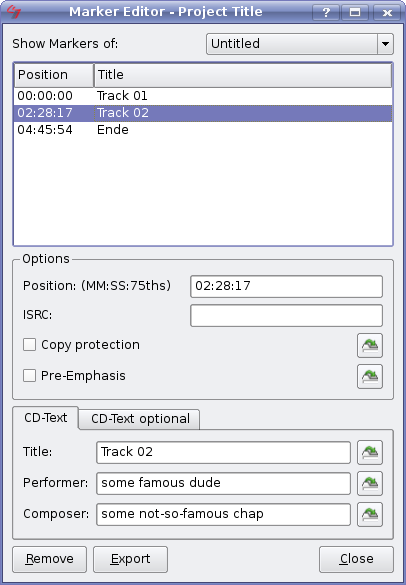
\includegraphics[width=0.45\textwidth]{images/marker-editor}
 \caption{The marker dialogue opened from ``Views $\rightarrow$ Marker Dialog'' allows to add CD-text, modify the markers, and export the table of contents as an HTML file.}
 \label{fig_marker-editor}
\end{figure}

Once the CD is laid out to your satisfaction, press \dact{RETURN} on the sheet to open the export dialogue (\FigB~\ref{fig_exportdlg}). You can either choose to export the project as audio files to the harddisk, or burn a CD. If you want to export to harddisk, you can choose between several audio formats. The most common one is WAVE, and depending on your plans with the exported files, you can use different sample formats (bit depths). 16 bit is ideal if you want to burn the files on CD later on. If you want to go on processing the files, use 32 bit float format instead. If you want to archive the files, use the FLAC codec, which is a lossless compression format.

If you want to burn a CD, you must also decide if you want to burn the current sheet (using markers to define CD tracks), or the entire project (each sheet becomes a track). If you check ``Export to disk only'', no CD will be written, but only a *.toc file and *.wav files for \texttt{cdrdao}.

Note for OS X users: CD writing support is still experimental. You can choose between several burning devices: IODVDServices, IODVDServices/2, IOCompactDiscServices, IOCompactDiscServices/2. These are hard-coded, so you probably don't have all of them installed. IOCompactDiscServices should only be used for old drives without DVD reading support. If you have multiple DVD drives, use IODVDServices or IODVDServices/2 to access the first and the second drive. In most cases IODVDServices will be the only working solution.

\begin{figure}[t]
 \centering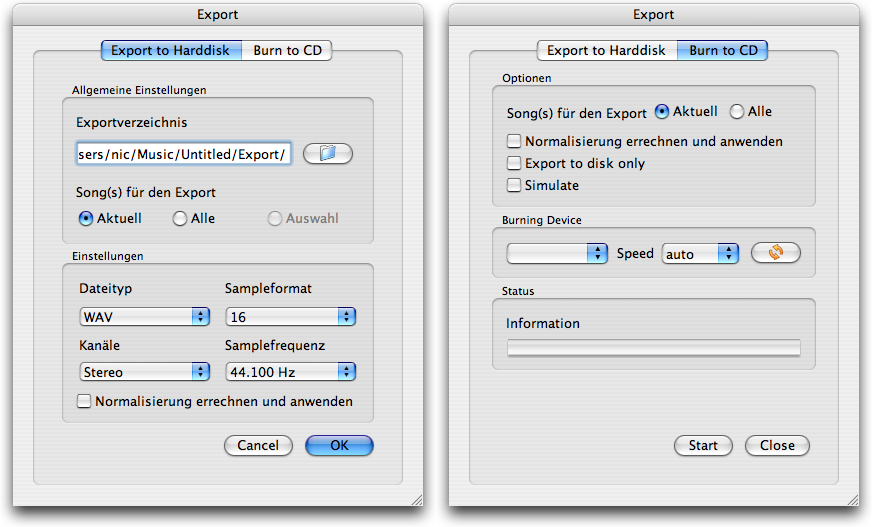
\includegraphics[width=\textwidth]{images/exportdlg}
 \caption{\dact{RETURN} opens a dialogue to export the project (either the current sheet or the entire project) to audio files, or burn a CD.}
 \label{fig_exportdlg}
\end{figure}

